\documentclass{article}
\usepackage{fullpage}
\usepackage{amsfonts}
\usepackage{amssymb}
\usepackage{amsmath}
\usepackage{hyperref}
\usepackage{graphicx}% Include figure files
\usepackage{epstopdf}
\usepackage{subfig}

%\usepackage{setspace}\doublespace
\author{Monique Combescot \and Guojun Zhu}
\title{Moth-eaten effect on BEC-BCS pairing}
\newcommand{\vk}{\ensuremath{\mathbf{k}}}
\newcommand{\vK}{\ensuremath{\mathbf{K}}}
\providecommand{\vr}{\ensuremath{\mathbf{r}}}
%\newcommand{\vec}[1]{\ensuremath{\mathbf{#1}}}

\newcommand{\gk}{\ensuremath{{g}(\mathbf{k})}}

\newcommand{\vp}{\ensuremath{\mathbf{p}}}
\newcommand{\gp}{\ensuremath{{g}(\mathbf{p})}}

\newcommand{\vq}{\ensuremath{\mathbf{q}}}

\newcommand{\Fo}{\ensuremath{\mathbf{F_0}}}


\newcommand{\E}{\ensuremath{\mathbf{E}}}
\newcommand{\A}{\ensuremath{\mathbf{A}}}
\newcommand{\J}{\ensuremath{\mathcal{J}}}

\newcommand{\ket}[1]{\ensuremath{\left|#1\right>}}
\newcommand{\bra}[1]{\ensuremath{\left<#1\right|}}

\newcommand{\twoe}{\ensuremath{2\epsilon_\vk-\E_1}}

\newcommand{\nth}[1]{\ensuremath{\frac{1}{#1}}}

\newcommand{\br}[1]{\ensuremath{\left(#1\right)}}
\newcommand{\mbr}[1]{\ensuremath{\left[#1\right]}}
\newcommand{\bbr}[1]{\ensuremath{\left\{#1\right\}}}


\newcommand{\tk}{\ensuremath{\tilde{k}}}

\newcommand{\kp}{\ensuremath{\ket{\Psi}}}

\newcommand{\av}[1]{\ensuremath{\bigl<{#1}\bigr>}}
\newcommand{\avs}[3] {\av{#1{\lvert{#2}\rvert}#3}}
\newcommand{\avv}[2][\nu] {\avs{#1}{#2}{#1}}
\newcommand{\avt}[2]{\av{{#1}|{#2}}}
\newcommand{\avtu}[1]{\av{T_\tau#1}}

\newcommand{\Bop}{\ensuremath{\mathbf{B_0^+}}}
\newcommand{\Bmp}{\ensuremath{\mathbf{B_m^+}}}
\newcommand{\Bnp}{\ensuremath{\mathbf{B_n^+}}}
\newcommand{\Bo}{\ensuremath{\mathbf{B_0}}}
\newcommand{\Bopn}{\ensuremath{\mathbf{{B_0^+}^n}}}
\newcommand{\Bon}{\ensuremath{\mathbf{{B_0}^n}}}


\newcommand{\zmatrix}{\ensuremath{\br{\begin{smallmatrix}0&0\\0&0\end{smallmatrix}}}}
\newcommand{\fmtrx}[4]{\ensuremath{\br{\begin{smallmatrix}#1&#2\\#3&#4\end{smallmatrix}}}}
\newcommand{\smtrx}[6]{\ensuremath{\br{\begin{smallmatrix}#1&#2\\#3&#4\\#5&#6\end{smallmatrix}}}}

\newcommand{\vz}{\ensuremath{v^{\beta\alpha}_{\vk,\vk}}}


\providecommand{\abs}[1]{\ensuremath{\lvert{#1}\rvert}}

\newcommand{\sg}[1][1]{\ensuremath{\sigma_\frac{#1}{2}}}

\newcommand{\rhof}{\ensuremath{\rho(\ef)}}
\newcommand{\omt}{\ensuremath{\tilde{\Omega}}}
\newcommand{\cht}{\ensuremath{\tilde{\chi_0}}}
\newcommand{\Atl}{\ensuremath{\abs{A}^{2l}}}
\newcommand{\ef}{\ensuremath{\epsilon_F}}

\newcommand{\lca}{\ensuremath{\ln\br{1+\frac{\cht}{\alpha}}}}

\newcommand{\com}[2]{\ensuremath{\mbr{#1,#2}}}
\newcommand{\D}{\ensuremath{\mathit{D}}}
\newcommand{\dg}{\ensuremath{\dagger}}
\newcommand{\nG}{\ensuremath{\hat{\mathcal{G}}^{-1}}}

\providecommand{\lvk}{\ensuremath{1/\vk_F}}
\providecommand{\hm}{\ensuremath{\frac{\hbar^2}}{2m}}
\providecommand{\pdiff}[2]{\ensuremath{\frac{\partial{#1}}{\partial{#2}}}}
\providecommand{\dpdiff}[2]{\ensuremath{\frac{\partial^2{#1}}{\partial{{#2}^2}}}}

\providecommand{\H}{\ensuremath{\mathcal{H}}}
\providecommand{\wt}[1]{\widetilde{#1}}

\providecommand{\eef}[1]{Eq. (\ref{#1})}

\providecommand{\sch}{{Schr\"{o}dinger }}

\providecommand{\sgn}{\ensuremath{\text{sgn}}}
\newcommand{\Arctg}{\ensuremath{\text{Arctg}}}

\providecommand{\comm}[1]{\textit{\scriptsize \uwave{(#1)}}}
\renewcommand{\emph}[1]{\textbf{#1}}
\newcommand{\td}{{\ensuremath{{\text{(2D)}}}}}
\newcommand{\sd}{{\ensuremath{{\text{(3D)}}}}}
\newcommand{\Arctg}{\ensuremath{\text{Arctg}}}
\begin{document}
\maketitle
\numberwithin{equation}{section}
\section{Introduction}
It is well-known that in 3D, a weak attractive potential cannot sustain a bound-state.  In 1956, Cooper demonstrated that with a frozen Fermi sea, a pair of electrons of opposite spin can form a bound-state comparing to the Fermi energy no matter how weak the attraction is\cite{Cooper}.  This is indeed a many-body state as Fermi sea, a fundamentally many-body phenomena,  is essential for the two-body ``bound state''.   The next year, Bardeen, Cooper and Schrieffer constructed a many-body ansatz which is an extension of this ``bound state'' and showed that this ansatz gives an intricate many-body state with lower energy than free Fermi gas with arbitrarily weak attraction\cite{BCS} for the same reduced BCS hamiltonian.  They used a particle-number non-conserved ansatz in a grand-canonical ensemble.  Nevertheless, the reduced BCS model also has a frozen Fermi sea in the core. Later,   Gallinskii et. al. showed that the frozen Fermi sea is not necessary and the same type of ansatz worked with a renomalized attraction measured by scattering amplitude\cite{}.   Furthermore, Eagles\cite{Eagles}, Leggett\cite{LeggettCrossover}, Nozi\`{e}res and Schmitt-Rink\cite{Nozieres} extended the BCS pairing idea and bridged BCS pairing and molecular BEC. There they used the model without a frozen Fermi sea as core and employed the full k-space.  All these lead to an interesting question that how the solution for the same hamiltonian evolves from one-pair, where there might be no bound state, to infinite number of pairs, where a many-body solution always exists.  Nevertherless, the particle non-conserved nature of the BCS ansatz makes it quite difficult to put both sides into the same footing.  

Five years after BCS, Richardson showed that a number-conserved eigenstate exists for reduced BCS Hamiltonian and it gives the same energy as BCS ansatz in thermaldynamic limit\cite{Richardson1,Richarson2,Richardson3,Richardson1968,gaudin}.  In the model, a frozen Fermi sea also exists in order to provide a constant density of states.  Since 2000, we developed a new theory for composite bosons (cobosons for short) formed by fermion pairs\cite{CobosonPhysicsReports} for electron excitons.   Recently, we applied it into superconductivity and it was proved to be useful.  We rederived Richardson-Gaudin equations with coboson framework\cite{CobosonBcsRich}. We also studied Richardson equations in details \cite{CombescotCooper,twoCooperPair}.  Richardson-Gaudin solution, as a number-conserved one, is just suitable to investigate the question we raised in previous paragraph.  

We illustrate our model in sec. \ref{sec:model}.  In sec. \ref{sec:onePair}, we study the one-pair problems in detail for both 2D and 3D.  We discussed the N-pairs problems, and make some conjecture about their connection with one-pair solution  in sec. \ref{sec:NPair}.  And we will attempt 2-pair Richardson-Gaudin equations and put the conjection into the solid ground in sec \ref{sec:twoPair}.  And we will offer some final thought in sec. \ref{sec:conclusion}.
\section{The system\label{sec:model}}
We consider $N$ fermion pairs $(\alpha,\beta)$ governed by the hamiltonian
\begin{equation}
H=H_{0}+V
\end{equation}
where $H_0$ is the kinetic energy 
\begin{equation}
H_0=\sum_{\vk}\epsilon_\vk(a^\dagger_\vk{}a^{}_\vk+b^\dagger_\vk{}b^{}_\vk)
\label{eq:}
\end{equation}
and $V$ is interaction
\begin{equation}
V=-v\sum_{\vk\vk'}\omega_{\vk'}\omega_\vk\beta^\dagger_{\vk'}{}\beta^{}_\vk
\label{eq:VBcs}
\end{equation}
and $\beta^\dagger_{\vk}=a^\dagger_{\vk}b^\dagger_{-\vk}$ creates a zero momentum pair while $\omega_\vk=1$ for $0<\epsilon_\vk<\Omega$ and zero otherwise.  
\section{One pair\label{sec:onePair}}
The single pair energy $E_1$ follows from Cooper equation
\begin{equation}
1=v\sum_{\vk}\frac{\omega_\vk}{2\epsilon_\vk-E_1}\equiv{}v\,S(E_1)
\label{eq:}
\end{equation}
\subsection{2D systems}
In 2D, the density of state is constant, so that 
\begin{equation}
S^{(\text{2D})}(E<0)=\rho\int_0^{\Omega}\frac{d\epsilon}{2\epsilon-E}=\frac{\rho}{2}\ln\left(\frac{2\Omega-E}{-E}\right)
\label{eq:}
\end{equation}
\begin{figure}[htbp]
	\centering
		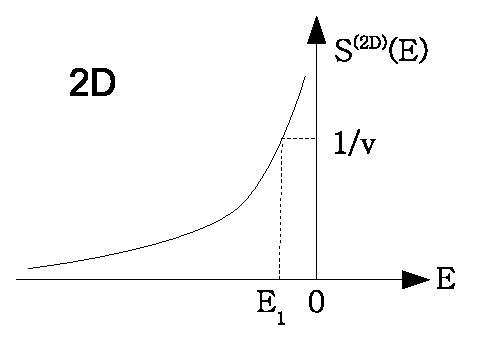
\includegraphics[width=0.30\textwidth]{2dOnePair.eps}
	\caption{$S^\td(E)$ function}
	\label{fig:2dOnePair}
\end{figure}

$S^{(\text{2D})}(E)$ diverges when $E\rightarrow{}0_{-}$ while it goes to zero as $\rho\Omega/(-E)$ when $E$ goes to $-\infty$. A bound state with $E_1<0$, thus exists no matter how weak $v$ is. It is given by 
\begin{equation}
E_1^{(\text{2D})}=-\frac{2\sigma}{1-\sigma}\Omega
\label{eq:}
\end{equation}
where $\sigma=e^{-2/\rho{v}}$



\subsection{3D systems}
In 3D, the density of states increases as $\sqrt{\epsilon}$. Let us write it as 
\begin{equation}
\rho(\epsilon)=\rho\sqrt{\epsilon/\Omega}
\label{eq:}
\end{equation}
where $\rho$ is the density of state at the potential threshold. We then have
\begin{equation}
\begin{split}
S^\sd(E<0)&=\rho\int_0^\infty{}d\epsilon\frac{\sqrt{\epsilon/\Omega}}{2\epsilon-E}\\
	&=\rho(1-\sqrt{\frac{-E}{2\Omega}}\Arctg\sqrt{\frac{2\Omega}{-E}})
\label{eq:}
\end{split}
\end{equation}
\begin{figure}[htbp]
	\centering
		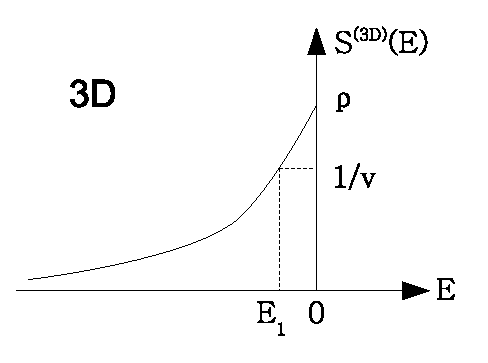
\includegraphics[width=0.30\textwidth]{3dOnePair.eps}
	\caption{$S^\sd(E)$ function}
	\label{fig:3dOnePair}
\end{figure}

$S^\sd(E)$ goes to $\rho$ when $E\rightarrow0_-$ while it goes to zero as $\frac{2}{3}\rho\Omega/(-E)$ when $E$ goes to $-\infty$. 

A bound state with $E_1<0$ thus exists for $v$ larger than the threshold value for $N=1$ pair $v_{\text{th}}=1/\rho$.  For a potential just above threshold, the single pair energy in 3D tens to zero as 
\begin{equation}
E_1^\sd\approx-\frac{8}{\pi^2}\left(1-\frac{v_{\text{th}}(N=1)}{v}\right)^2\Omega
\label{eq:}
\end{equation}
while for a potential far above threshold $E_1^\sd$ behaves as 
\begin{equation}
E_1^\sd\approx-\frac{2}{3}\frac{v}{v_\text{th}^{\text{(1)}}}\Omega
\label{eq:}
\end{equation}


\section{N pairs\label{sec:NPair}}
Richardson \cite{Richardson1} and Gaudin \cite{gaudin} have shown that the energy of N fermion pairs interacting through the BCS reduced potential is exactly given by $E_N=R_1+\cdots+R_N$ where the $R_i$'s follow from $N$ coupled nonlinear equations
\begin{equation}
 1=v\sum_\vk\frac{w_\vk}{2\epsilon_\vk-R_i}+\sum_{j\neq{}i}\frac{2v}{R_i-R_j}\qquad\text{for}\;i=(1,\cdots,N)
\end{equation}
\subsection{2D systems}
We have shown that when the density of states is constant, as in standard BCS superconductivity set also in 2D systems, a compact form of $E_N$ can be derived. It leads to 
\begin{equation}
 E^(2D)_N=N\,E^{2D}_1+\frac{N(N-1)}{\rho}\frac{1+\sigma}{1-\sigma}
\end{equation}
within under extensive terms in $(N/\rho)^n$ with $n\leq2$

This gives the condensation energy in $N$ pairs, i.e., the difference between the $N$-pair energy without and with potential, as 
\begin{equation}\label{eq:E2D}
\begin{split}
 \mathcal{E}^{(2D)}_N&=E_N^{\td}(v=0)-E_N^\td\equiv{}N\epsilon_N^\td\\
&=N(1-\frac{N-1}{N_\Omega})\frac{2\sigma}{1-\sigma}\Omega
\end{split}
\end{equation}
where $N_\Omega=\rho\Omega$ is the number of states in the potential layer. 

The condensation energy per pair $\epsilon^\td_N=\mathcal{E}^\td_N/N$ thus decreases linearly with N. This decrease is due to a moth-eaten effect induced by Pauli blocking on the number empty states feeling the potential and thus available to from the $N$-pair bound state.  In the limit of a number of pairs filling the potential layer, $N=N_\Omega$, the condensation energy reduceds to 
\begin{equation}
 \mathcal{E}^\td_{N_\Omega}=\Omega[\frac{2\sigma}{1-\sigma}]
\end{equation}
so that the condensation energy per pair tends to zero as $\epsilon^\td_{N_\Omega}=[2\sigma/(1-\sigma)]/\rho$ in the large sample limit: for $N=N_\Omega$, the system has no more freedom to construct a lower energy ground state, the condensation energy per pair thus have to cancel.  


\begin{figure}[htbp]
	\centering
		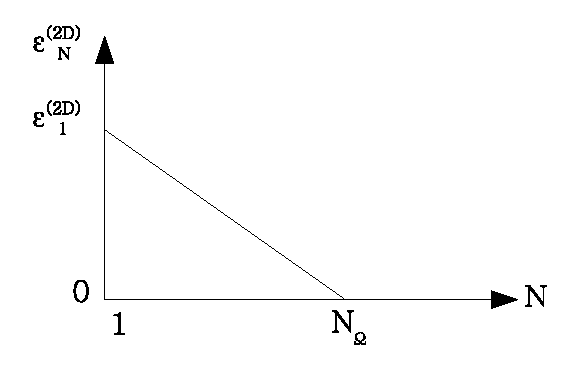
\includegraphics[width=0.30\textwidth]{2dCondEnergy.eps}
	\caption{Condensation Engery Change  with Pair Numbers in 2D}
	\label{fig:2dCondEnergy}
\end{figure}



\subsection{3D system}
A similar compact expression of the $N$-pair energy has not been derived so far in the case of a $\sqrt{\epsilon}$ density of states. Let us first qualitatively understand the behavior of the $N$ pair energy when $N$ increases. 

It is clear that the same moth eaten effect must bring the condensation energy per pair down to zero when $N$ approach $N_\Omega$, this effect fundamentally linked to the Pauli exclusion principle being unaffected by an increase of space dimensionality. 

\subsubsection{}
For potential $v$ lower than the threshold value $v_{th}(1)=1/\rho$ for the existence of one-pair bound state, $\mathcal{E}_N^\sd$ is equal to zero for $N=1$ and also for $N=N_\Omega$.  It is however clear that $\mathcal{E}_N^\sd$ cannot stay equal to zero for all $N$ between $1$ and $N_\Omega$ because for $N$ equal to a praction of $N_\Omega$, the density of states is essentially constant.  So that we can at least freeze a fraction of the $N$ electrons as in standard BCS superconductivity with a frozen core: a finite condensation thus exists no matter how weak $v$ is. 

\begin{figure}[htbp]
	\centering
		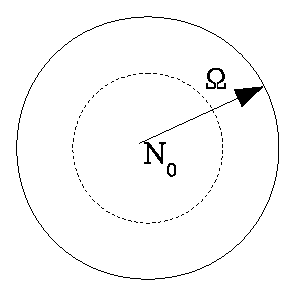
\includegraphics[width=0.30\textwidth]{potential.eps}
	\caption{Imaginary Frozen Core for Many Pairs in 3D}
	\label{fig:potential}
\end{figure}

We can have a lower boundary of this condensation energy per pair by freezing $N_0$ of these $N$ electrons.  The remaining $N-N_0$ pairs enjoy the potential attraction in a region where the/852 density of state stays finite, between $\rho\sqrt{\epsilon_{F_0}/\Omega}$ and $\rho$.  The condensation energy of these $(N-N_0$ pairs would then read according to Eq. (\ref{eq:E2D})
\begin{equation}\label{eq:E2D}
 \overline{\mathcal{E}}_{N-N_0}=(N-N_0)(1-\frac{N-N_0-1}{N_\Omega})\frac{2\bar\sigma}{1-\bar\sigma}\Omega
\end{equation}
where $\bar{\sigma}=e^{-2/{\bar{\rho}v}}$ with $\bar\rho$ being average density of states in the potential layer above the frozen core. This gives a condensation energy per pair equal to $\overline{\mathcal{E}}_{N-N_0}/N$.  By taking $\bar\rho$ as independent of $N_0$, we find that this condensation energy per pair is maximized at $N-N_0=N_\Omega/2$, which of course implies to have $N$ larger than $N_\Omega/2$.

This argument actually shows that, even if $N$ is not as large as $N_\Omega/2$, but still a sizable faction of the total number of pair state $N_\Omega$ feeling the potential,  a BCS-like collective effect develops which produces a non-zero condensation energy no matter how weak the potential is, i.e., even for $v\ll{}v_\text{th}(1)$. 

As a result, the threshold potential for the appearance of a $N$-pair bound state must decrease with $N$, down to eventually zero with $N$ is a sizable fraction of the total number of pairs $N_\Omega$ in the potential layer. 

\begin{figure}[htb]
	\centering
		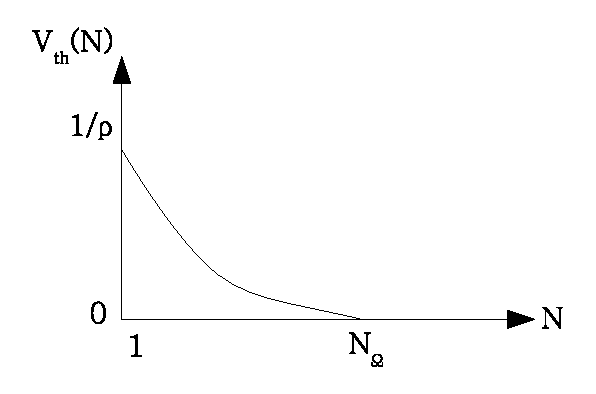
\includegraphics[width=0.30\textwidth]{3dThresholdChange.eps}
	\caption{Threshold change against number of pairs in 3D}
	\label{fig:3dThresholdChange}
\end{figure}

\subsubsection{}
For $v$ just larger than the threshold value $v_{\text{th}}(1)=1/\rho$ for the appearance of ground state in case of only one pair, it is clear by continuity, that the condensation energy per pair $\epsilon^sd_N$, must first increases with $N$ and then decreases due to the moth-eaten effect which must end by controlling the behavior of $\epsilon_N$ when $N$ approaches $N_\Omega$.  Although fully reasonable, the fact that the behavior of $\epsilon^\sd_N$ must continuous and thus first increases when $v$ gets above $v_{\text{th}}(1)$ is a mathematical argument, not a physical argument. 

It is actually possible to guess the physical origin of the condensation energy increase when $N$ departs from 1.  For that, we have to remember that the ``condensation energy is difference of two energies which go to increase with $N$ due to Pauli blocking.  The question then is to understand why, for small $N$, the free pair energy increases faster than the correlated pair energy.  When on free pair is added at the energy level $\epsilon$, the kinetic energy increases by $1/\rho(\epsilon)$.  As a result, in 3D systems with density of states $\sqrt{\epsilon}$, the free pair energy increase, when going from $N$ to $N+1$ pairs, is larger when the Pauli exclusion principle blocks a low energy then a state high in the band.  If we now turn to correlated pairs, we must note that theses are made of all pairs in the potential layer. When increasing their number from $N$ to $N+1$, we blocks a very small fraction of each of the states between $0$ and $\Omega$, so that the energy cost must be far less than when blocking a single low energy state.  Consequently the energy difference when adding one free pair on one correlated must increase with $N$ is small. By contrast when $N$ gets larger, the cost in energy $1/\rho(\epsilon)$ to add one free pair is eventually constant and equal to the cost to block any of the $\vk$ states making the correlated pair.  We are then left with the moth-eaten effect on the bound state itself which tends to decrease the condensation energy. 

This understanding is supported by the monotonous decrease of the condensation energy per pair we find in 2D: the density of state being constant, the energy cost to block a single low energy state is the same as for any of the states making the correlated pair so that we only feel the moth-eaten effect on the number of states available to construct the correlated configuration.  As a result, the condensation energy per pair has to decrease without when $N$ increases as we find.  

In order to establish this qualitative understanding on strong grounds, let us consider $N=2$ pairs. This limiting case gives the trend of the $N$ dependence of the condensation energy since it actually contains the physics which drives this $N$ dependence, namely Pauli blocking.  


\section{Condensation energy in two pairs\label{sec:twoPair}}
The exact energy of two fermion pairs in the BCS potential gives in Eq. (\ref{eq:VBcs}) has been shown to read $E_2=R_1+R_2$ with $(R_1,R_2)$ solution of the two Richardson-Gaudin equations
\begin{equation}
\begin{split}
1&=v\sum_{\vk}\frac{w_\vk}{2\epsilon_\vk-R_1}+\frac{2v}{R_1-R_2}\\
1&=v\sum_{\vk}\frac{w_\vk}{2\epsilon_\vk-R_2}+\frac{2v}{R_2-R_1}
\end{split}
\label{eq:richardsonEq}
\end{equation}

\begin{figure}[htb]
	\centering
		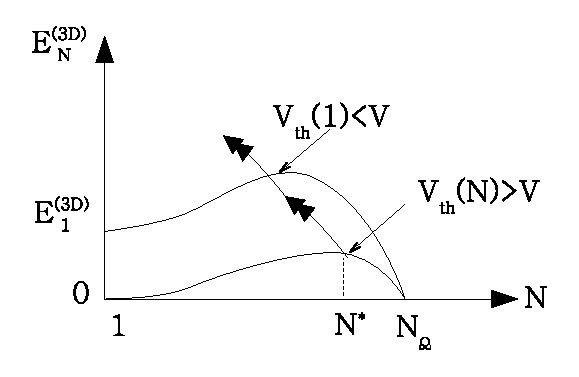
\includegraphics{3dCondChange.eps}
	\caption{Condensation energy change with number of pairs in 3D}
	\label{fig:3dCondChange}
\end{figure}

We have been able to solve these coupled equations analytically in the case of a constant density of states\cite{twoCooperPair}.  Using this work, we find the for 2D systems with $w_\vk=1$ for $0<\epsilon_k<\Omega$, the energy difference between two correlated pairs and two independent pairs reads in the larger sample limit, as 
\begin{equation}
E^{\td}_2-2E_1^{\td}=\frac{2}{\rho}\frac{1+\sigma}{1-\sigma}+\text{O}(\frac{1}{\rho^2})
\label{eq:}
\end{equation}
the $2/\rho$ part of this difference is the kinetic energy cost to add one pair while $2[2\sigma/(1-\rho)]$ is the energy in the binding energy of two pairs induced by the moth-eaten effect. This result far easier to obtain than the one for arbitrary $N$, not only gives the trend induced by Pauli blocking on the energy of $N$ correlated pairs, but also allow to obtain this energy exactly through a rule of the thumb that we have learned valid for all exciton problems we have studied up to now -excitons also are composite bosons with a many-body physics driven by Pauli blocking.  This rule says that, in the thermodynamical limit, i.e., large volume but $N\\rho$ constant, the result for $N$ is the result in 2 multiplied by $N-1$.  In the present case, this gives the energy change per pair, $[E^{\td}_N-NE^{\td}_1]/N$, as $[(N-1)/\rho](1+\sigma)/(1-\sigma)$ in agreement with the result we have found through far more complicated calculation than the ones for just $N=2$.

We are here interested in finding the solution of these two equations when free density of states is not constant but varies as $\rho\sqrt{\epsilon/\Omega}$.  Since the solution of these equations for $N=1$, i.e., without the $2v/(R_1-R_2)$ terms in Eq. (\ref{eq:richardsonEq}), dramatically depends on the value of $v$, with no ground state, i.e., negative solution, when $v$ is smaller than $v_{\text{th}}(1)=1\rho$, we are led to consider the three cases $v\rho>1$, $v\rho<1$ and $v\rho=1$ separately. 

Actually, a property of the $R_i$'s we have found in our previous work, is still valid whatever $\rho{}v$ is, namely the fact that $R_1$ and $R_2$ are both complex with $R_1=R_2^*$ is order to have $R_1+R_2=E_2$ real.  Let us first reproduce the argument in completeness. 

\subsection{$(R_1,R_2)$ are complex conjugate}
XXXXXXXXXXXXXXXXXXXXXXXXXXXXXXXXXXX
\subsection{Solution in $v\rho=1$}
Let us start with the threshold case $v=v_{\text{th}}(1)$, i.e., $v\rho=1$.  We then have $S(E=0)=1$, so that the Richardson-Gaudin equations also read, for $R_1=R+iR'$
\begin{equation}
\sum\frac{w_\vk}{2\epsilon_\vk}=\sum\frac{w_\vk}{2\epsilon_\vk-R-iR'}-\frac{i}{R'}
\label{eq:}
\end{equation}
This equation splits into two equations, for the real and imaginary parts

The problem then is to find $R$ solution of 
\begin{equation}
\sum\frac{w_\vk}{2\epsilon_\vk}=\sum{}w_\vk\frac{2\epsilon_\vk-R}{(2\epsilon_\vk-R)^2+R'^2}
\label{eq:}
\end{equation}
where $R'$ such that 
\begin{equation}
R'^2\sum{}\frac{w_\vk}{(2\epsilon_\vk-R)^2+R'^2}=1
\label{eq:R'}
\end{equation}
in the large sample limit, i.e., the dominate term of the $\rho$ dependence of $R$ wehn $1/\rho$ goes to zero. 

By combining these two equation, we get
\begin{equation}
R\sum{}w_\vk\frac{2\epsilon_\vk-R}{(2\epsilon_\vk-R)^2+R'^2}=1
\label{eq:R}
\end{equation}

A possible trick to solve these equations is to note that $\sum_\vk{}w_\vk=N_\Omega=\frac23\rho\Omega$ in 3D (which it is $\rho\Omega$ in 2D).  This allows to rewrite Eqs. (\ref{eq:R'},\ref{eq:R})
\begin{gather}
\sum{}w_\vk\left[\frac{1}{(2\epsilon_\vk-R)^2+R'^2}-\frac{1}{N_\Omega{}R'^2}\right]=0\\
\sum{}w_\vk\left[\frac{2\epsilon_\vk-R}{(2\epsilon_\vk-R)^2+R'^2}-\frac{1}{N_\Omega{}R}\right]=0
\end{gather}
This readily shows that if $R$ and $R'$ were finite when $\rho\rightarrow\infty$, i.e., these queation cannot be fulfilled because we 

\section{conclusion\label{sec:conclusion}}

\bibliography{../citation}
%\bibliographystyle{apsrmp4-1long}
\bibliographystyle{apalike}

\end{document}
